Um eine webbasierte Anwendung zu erstellen, die ohne einen zentralen Server auskommt, muss die Software komplett clientseitig in einem Browser ausgeführt werden und damit auch zwangsläufig in JavaScript implementiert werden. Ein klassisches Backend, also eine Datenschicht (üblicherweise handelt es sich bei den meisten Web-Applikationen mindestens um eine Zwei-Schichten-Architektur) existiert nicht, beziehungsweise ist in die Präsentationsschicht integriert. Das bedingt die Kategorisierung der entstehenden Anwendung als „Fat Client“.

Durch die vollständig clientseitige Ausrichtung bietet es sich an, die Software als sogenannte Single-Page-Application (SPA) zu implementieren. Herkömmliche Webseiten, sogenannte Multi-Page-Applications (MPA) laden während ihrer Lebenszeit mehrfach neue Seiten vom Server, zum Beispiel jedes Mal, wenn innerhalb der Anwendung eine neue Ansicht dargestellt werden soll. Eine SPA dagegen lädt nur eine einzige Webseite sowie das zugehörige JavaScript-Programm und verändert diese eine Seite dann im weiteren Verlauf dynamisch. Neue Daten werden bei Bedarf asynchron (ohne Blockieren der Seite) nachgeladen, es wird jedoch keine komplette Seite geladen. Damit wird auch eine maximale Autarkie gegenüber dem Webserver erreicht, da dieser nur mit wenigen Requests (im einfachsten Fall ein Request pro Nutzer) umgehen muss. Die Anforderungen an den Webserver, auf dem die Anwendung bereitgestellt wird, sind sehr gering – er muss lediglich statische Dateien (HTML, JavaScript, Bilder, Schriften, etc.) bereitstellen.

Als Framework für die Implementierung einer solchen SPA wird das React-Framework\cite{web:react} ausgewählt. Das Open-Source-Projekt existiert seit 2013 und wird von Facebook finanziert und gefördert. Es gehört zu den populärsten Frameworks zum Erstellen von Benutzeroberflächen und Web-Applikationen\cite{web:stackoverflow_umfrage} und ist dem Autor der Arbeit bereits vertraut.

Um einige Implementationsdetails nachzuvollziehen, erfolgt an dieser Stelle eine  Einführung in einige Grundkonzepte von React.

\subsection{Komponenten und State}
Die elementaren Bausteine einer React-Anwendung sind \texttt{Komponenten}. Die React-Dokumentation beschreibt die Aufgabe von Komponenten wie folgt\cite{web:react}:
\begin{quotation}
„Build encapsulated components that manage their own state, then compose them to make complex UIs.“
\end{quotation}

Ein Komponente ist eine autarke und wiederverwendbare Einheit und kapselt meistens sowohl Struktur, Aussehen als auch Logik. Komponenten werden häufig als Klasse implementiert (können aber in einfachen Fällen auch als Funktion implementiert werden) und erben von der Klasse \texttt{React.Component}. Valide Komponenten müssen über eine \texttt{render()}-Funktion verfügen, die HTML oder andere React-Komponenten zurückliefert. Eine sehr simple, statische Komponente könnte so aussehen:

\begin{minipage}{\linewidth}
\begin{lstlisting}[caption={Einfache React-Komponente ohne JSX-Syntax.}]
import React from "react";

class Greeting extends React.Component {
  render() {
    return React.createElement("div", null, "Hello there!");
  }
}
\end{lstlisting}
\end{minipage}

Da die Syntax des Aufrufs \texttt{React.createElement()} nicht so schön zu lesen ist, wie die Notation eines XML-Tags (\texttt{<div>...</div>}) wird im React-Umfeld üblicherweise eine Syntax-Erweiterung namens JSX (JavaScript Syntax Extension) verwendet, um React-Komponenten einfacher beschreiben zu können. JSX wird mit einem Compiler während des Build-Prozesses in herkömmliches JavaScript umgewandelt. Äquivalent zum letzten Beispiel wäre daher die folgende Variante unter Einbeziehung von JSX-Syntax:

\begin{minipage}{\linewidth}
\begin{lstlisting}[caption={Einfache React-Komponente mit JSX-Syntax.}]
import React from 'react';

class Greeting extends React.Component {
    render() {
        return <div>Hello there!</div>;
    }
}
\end{lstlisting}
\end{minipage}

Um Komponenten dynamisch zu machen, können über sogenannte \texttt{Properties} Daten an Komponenten übergeben werden. Auf diese kann mit dem \texttt{props}-Objekt zugegriffen werden:

\begin{minipage}{\linewidth}
\begin{lstlisting}[caption={Komponenten erhalten Daten über ihre Properties.}]
import React from "react";

class Greeting extends React.Component {
  render() {
    return <div>Hello, {this.props.name}!</div>;
  }
}
\end{lstlisting}
\end{minipage}

Properties werden wie andere HTML-Attribute auch einfach hinter den Namen einer Komponente innerhalb des zugehörigen Tags in die Instanziierung einer Komponente integriert:

\begin{minipage}{\linewidth}
\begin{lstlisting}[caption={Properties werden wie normale HTML-Attribute verwendet.}]
import React from "react";

class GreetAllFriends extends React.Component {
  render() {
    return (
      <div>
        <Greeting name="Michael" />
        <Greeting name="Karla" />
      </div>
    );
  }
}
\end{lstlisting}
\end{minipage}

\texttt{Properties} werden also verwendet, um Daten in Komponenten hinein zu reichen. React kümmert sich dann automatisch um das Aktualisieren der Ansicht, sobald sich eine Property ändert (dieses „reaktive“ Prinzip ist auch der Namensgeber für das Framework). Dabei verwendet React sehr schnelle und intelligente Algorithmen, um immer nur diejenigen Elemente einer Seite zu aktualisieren, die sich auch tatsächlich geändert haben. Dadurch können Single-Page-Applications schneller agieren als Multi-Page-Applications.

Properties können nicht modifiziert werden – sie sind wie auch die meisten anderen Objekte innerhalb von React „immutable“. Wenn Daten innerhalb einer Komponente modifiziert werden sollen, gehören sie in das interne, modifizierbare \texttt{state}-Objekt dieser Komponente:

\begin{minipage}{\linewidth}
\begin{lstlisting}[caption={Jede Komponente kann über einen modifizierbaren state verfügen.}]
import React from "react";

class BusyOrNot extends React.Component {
  state = {
    busy: false
  };

  toggleBusy() {
    this.setState(prevState => ({
      busy: !prevState.busy
    }));
  }

  render() {
    return (
      <div>
        <div>This user is {busy ? "busy" : "not busy"}!</div>
        <button type="button" onClick={this.toggleBusy}>
          Change Busy State
        </button>
      </div>
    );
  }
}
\end{lstlisting}
\end{minipage}

Bedingt durch die statische Natur der Properties, forciert React einen unidirektionalen Datenfluss. Daten können nur von „oben nach unten“ (in Bezug auf die Baumstruktur im Document-Object-Model einer Seite) durch eine Anwendung fließen. Möchten zwei Komponenten an unterschiedlichen Stellen auf die gleichen Daten zugreifen, dann sollten diese oberhalb der beiden Komponenten in einer gemeinsamen Eltern-Komponente gehalten werden.\newline

\begin{minipage}{\linewidth}
\begin{lstlisting}[caption={„Lifting state up“: Mehrere Komponenten greifen auf die gleichen Daten zu.}]
import React from "react";

function Son(props) {
  return <p>I am the son of {props.parent}</p>
}

function Daughter(props) {
  return <p>I am the daughter of {props.parent}</p>
}

class Parent extends React.Component {
  state = {
    parentName: "Peter Parent"
  };

  render() {
    return (
      <div>
        <Son parent={this.state.parentName} />
        <Daughter parent={this.state.parentName} />
      </div>
    );
  }
}
\end{lstlisting}
\end{minipage}

Da dieses Muster bei großen Anwendungen aber schnell zu sehr aufwendigem „Durchstecken“ von Properties (sogenanntes „Prop Drilling“) durch mehrere Komponenten-Ebenen führt, gibt es eine populäre Erweiterung für React zur Verwaltung eines einzigen, globalen States in der gesamten Anwendung: das Flux-Muster\cite{web:flux_doku}.


\subsection{State Management mit Redux}
\label{chap:redux_state_management}
Das Flux-Entwurfsmuster ist ebenfalls eine Entwicklung von Facebook. Prinzipiell handelt es sich um ein abstraktes Entwurfsmuster, das in vielen Sprachen angewendet werden kann. Etabliert hat es sich jedoch gerade in Kombination mit React-Anwendungen. Die bekannteste Implementation, die auch in dieser Arbeit verwendet wird, hört auf den Namen Redux\cite{web:redux}.

Im Flux-Muster geht es darum, eine zentrale Zustandsverwaltung für eine Anwendung einzurichten, eine sogenannte „Single Source of Truth“. Dieser zentrale Ort wird als \texttt{Store} bezeichnet. Ein Store beinhaltet typischerweise solche Daten, die für die gesamte Anwendung relevant sind. Parallel dazu kann es aber weiterhin Komponenten geben, die einen eigenen, lokalen State verwalten, wenn dieser nicht für die gesamte Anwendung relevant ist.

\begin{figure}[H]
    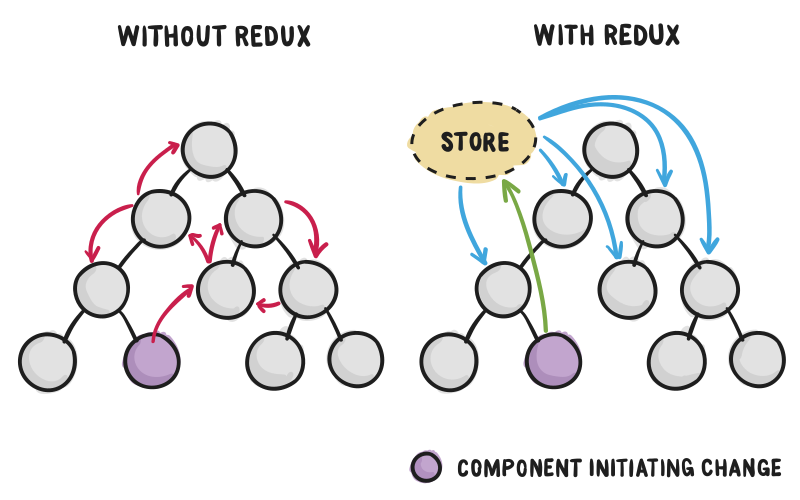
\includegraphics[width=12cm]{chapter/entwurf/bilder/BA_redux.png}
    \centering
    \caption{Der Redux-Store verwaltet den globalen Zustand einer React-Anwendung und ist die „Single Source of Truth“. Quelle: https://css-tricks.com/learning-react-redux/ (aufgerufen am 24.4.19)}
    \label{abb:redux_flow}
\end{figure}


Einzelne React-Komponenten können mit einem Store durch einen Publish/Subscribe-Mechanismus verbunden werden. In Redux wird diese Verbindung durch die \texttt{connect}-Funktion zur Verfügung gestellt. Die gewünschten Daten aus dem Store können in einer \texttt{mapStateToProps}-Funktion angegeben werden und stehen der Komponente dann als Properties zur Verfügung. Ändern sich die Daten im Store, dann wird die verbundene Komponente sofort benachrichtigt und bei einer Änderung der Properties auch neu gerendert (reaktives Prinzip). Um eine möglichst lose Kopplung zwischen den Komponenten zu realisieren, wird deswegen empfohlen, die Verbindung zu einem Store in einer (nicht sichtbaren) Container-Komponente zu realisieren. Im folgenden Beispiel wird die eigentliche, sichtbare \texttt{Header}-Komponente mit einem unsichtbaren Container versehen, der die notwendigen Daten aus dem Store innerhalb der Komponente unter der \texttt{status}-Property verfügbar macht.

\begin{minipage}{\linewidth}
\begin{lstlisting}[caption={Über den connect-Aufruf beim Exportieren der Komponente wird sie mit dem Store verbunden. (aus:  src/client/components/ClientHeaderContainer.js)}]
import { connect } from "react-redux";
import Header from "./Header";

const mapStateToProps = state => ({
  status: state.connection.status
});

export default connect(mapStateToProps)(Header);
\end{lstlisting}
\end{minipage}

Änderungen in einem Store müssen mithilfe von \texttt{Actions} realisiert werden. Bei einer Action handelt es sich lediglich um ein Objekt, welches die Art der Änderung in einem Store beschreibt. Um das wiederholte Schreiben solcher aufwändigen Objekt-Literale zu erleichtern, werden die Actions üblicherweise von einer einfachen \texttt{ActionCreator}-Funktion erzeugt:

\begin{minipage}{\linewidth}
\begin{lstlisting}[caption={Ein Action-Objekt ist lediglich die Beschreibung einer Änderungsoperation und wird in einem ActionCreator erzeugt.}]
export function addQuestion(newQuestion) {
  return {
    type: "ADD_QUESTION",
    payload: {
      newQuestion
    }
  };
}
\end{lstlisting}
\end{minipage}

Die eigentliche Implementierung einer Änderungsoperation erfolgt in dem zugehörigen \texttt{reducer}. Die Operationen in einem reducer sind stets pure Funktionen, das heißt, sie liefern immer das gleiche Ergebnis bei gleichen Eingabe-Parametern und sie haben keine Seiteneffekte. Die Parameter des reducers sind immer der aktuelle State des Stores und die eingehende Action, der Rückgabewert ist der neue State des Stores. Ein einfacher Reducer zum Hinzufügen einer Frage zu einem Fragekatalog könnte so aussehen:

\begin{minipage}{\linewidth}
\begin{lstlisting}[caption={In einem Reducer werden die Änderungsoperationen eines Stores als pure Funktion implementiert.}]
const questionEditor = (state = [], action) => {
  switch (action.type) {
    case "ADD_QUESTION": {
      return [... state, createNewQuestion()];
    }
  }
};
\end{lstlisting}
\end{minipage}

\subsection{Konkrete Umsetzung am Beispiel des Fragen-Editors}
Um das neue CRS zu implementieren, muss zunächst eine sinnvolle Aufteilung in React-Komponenten erfolgen. Exemplarisch soll an dieser Stelle einer der Hauptbestandteile der Anwendung besprochen werden: der Fragen-Editor.

Das zweiteilige Design, bestehend aus einer Fragenliste in der Seitenspalte und einem Fragen-Inhaltsbereich, das sowohl bei StuReSy als auch bei Pingo zum Einsatz kommt, soll beibehalten werden.

Eine mögliche Komponenten-Hierarchie für den Fragen-Editor wird in Abbildung \ref{abb:komponenten_hierarchie} veranschaulicht. Die äußerste Komponente, der \texttt{QuestionEditorContainer}, ist nicht sichtbar. Es handelt sich dabei lediglich um eine Container-Komponente, welche die notwendigen Daten aus dem Store holt und dann an ihre Kinder-Komponenten mittels Properties weitergibt.

\begin{figure}[H]
    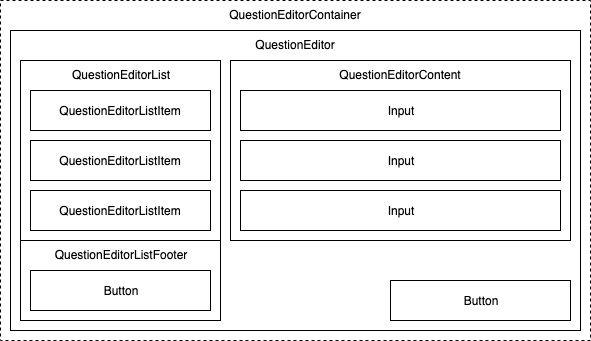
\includegraphics[width=\textwidth]{chapter/entwurf/bilder/Component_Hierarchy.png}
    \centering
    \caption{Mögliche Komponenten-Hierarchie für den Fragen-Editor.}
    \label{abb:komponenten_hierarchie}
\end{figure}

Die tatsächliche Implementierung entspricht nahezu vollständig diesem Bild (einzig die Komponente \texttt{QuestionEditorListItem} wurde aus Gründen der Drag-and-Drop-Funktionalität in der Seiteleiste nicht genau so implementiert).


\begin{figure}[H]
    \centering
    \setlength{\fboxsep}{0pt}
    \setlength{\fboxrule}{0.5pt}
    \fbox{
    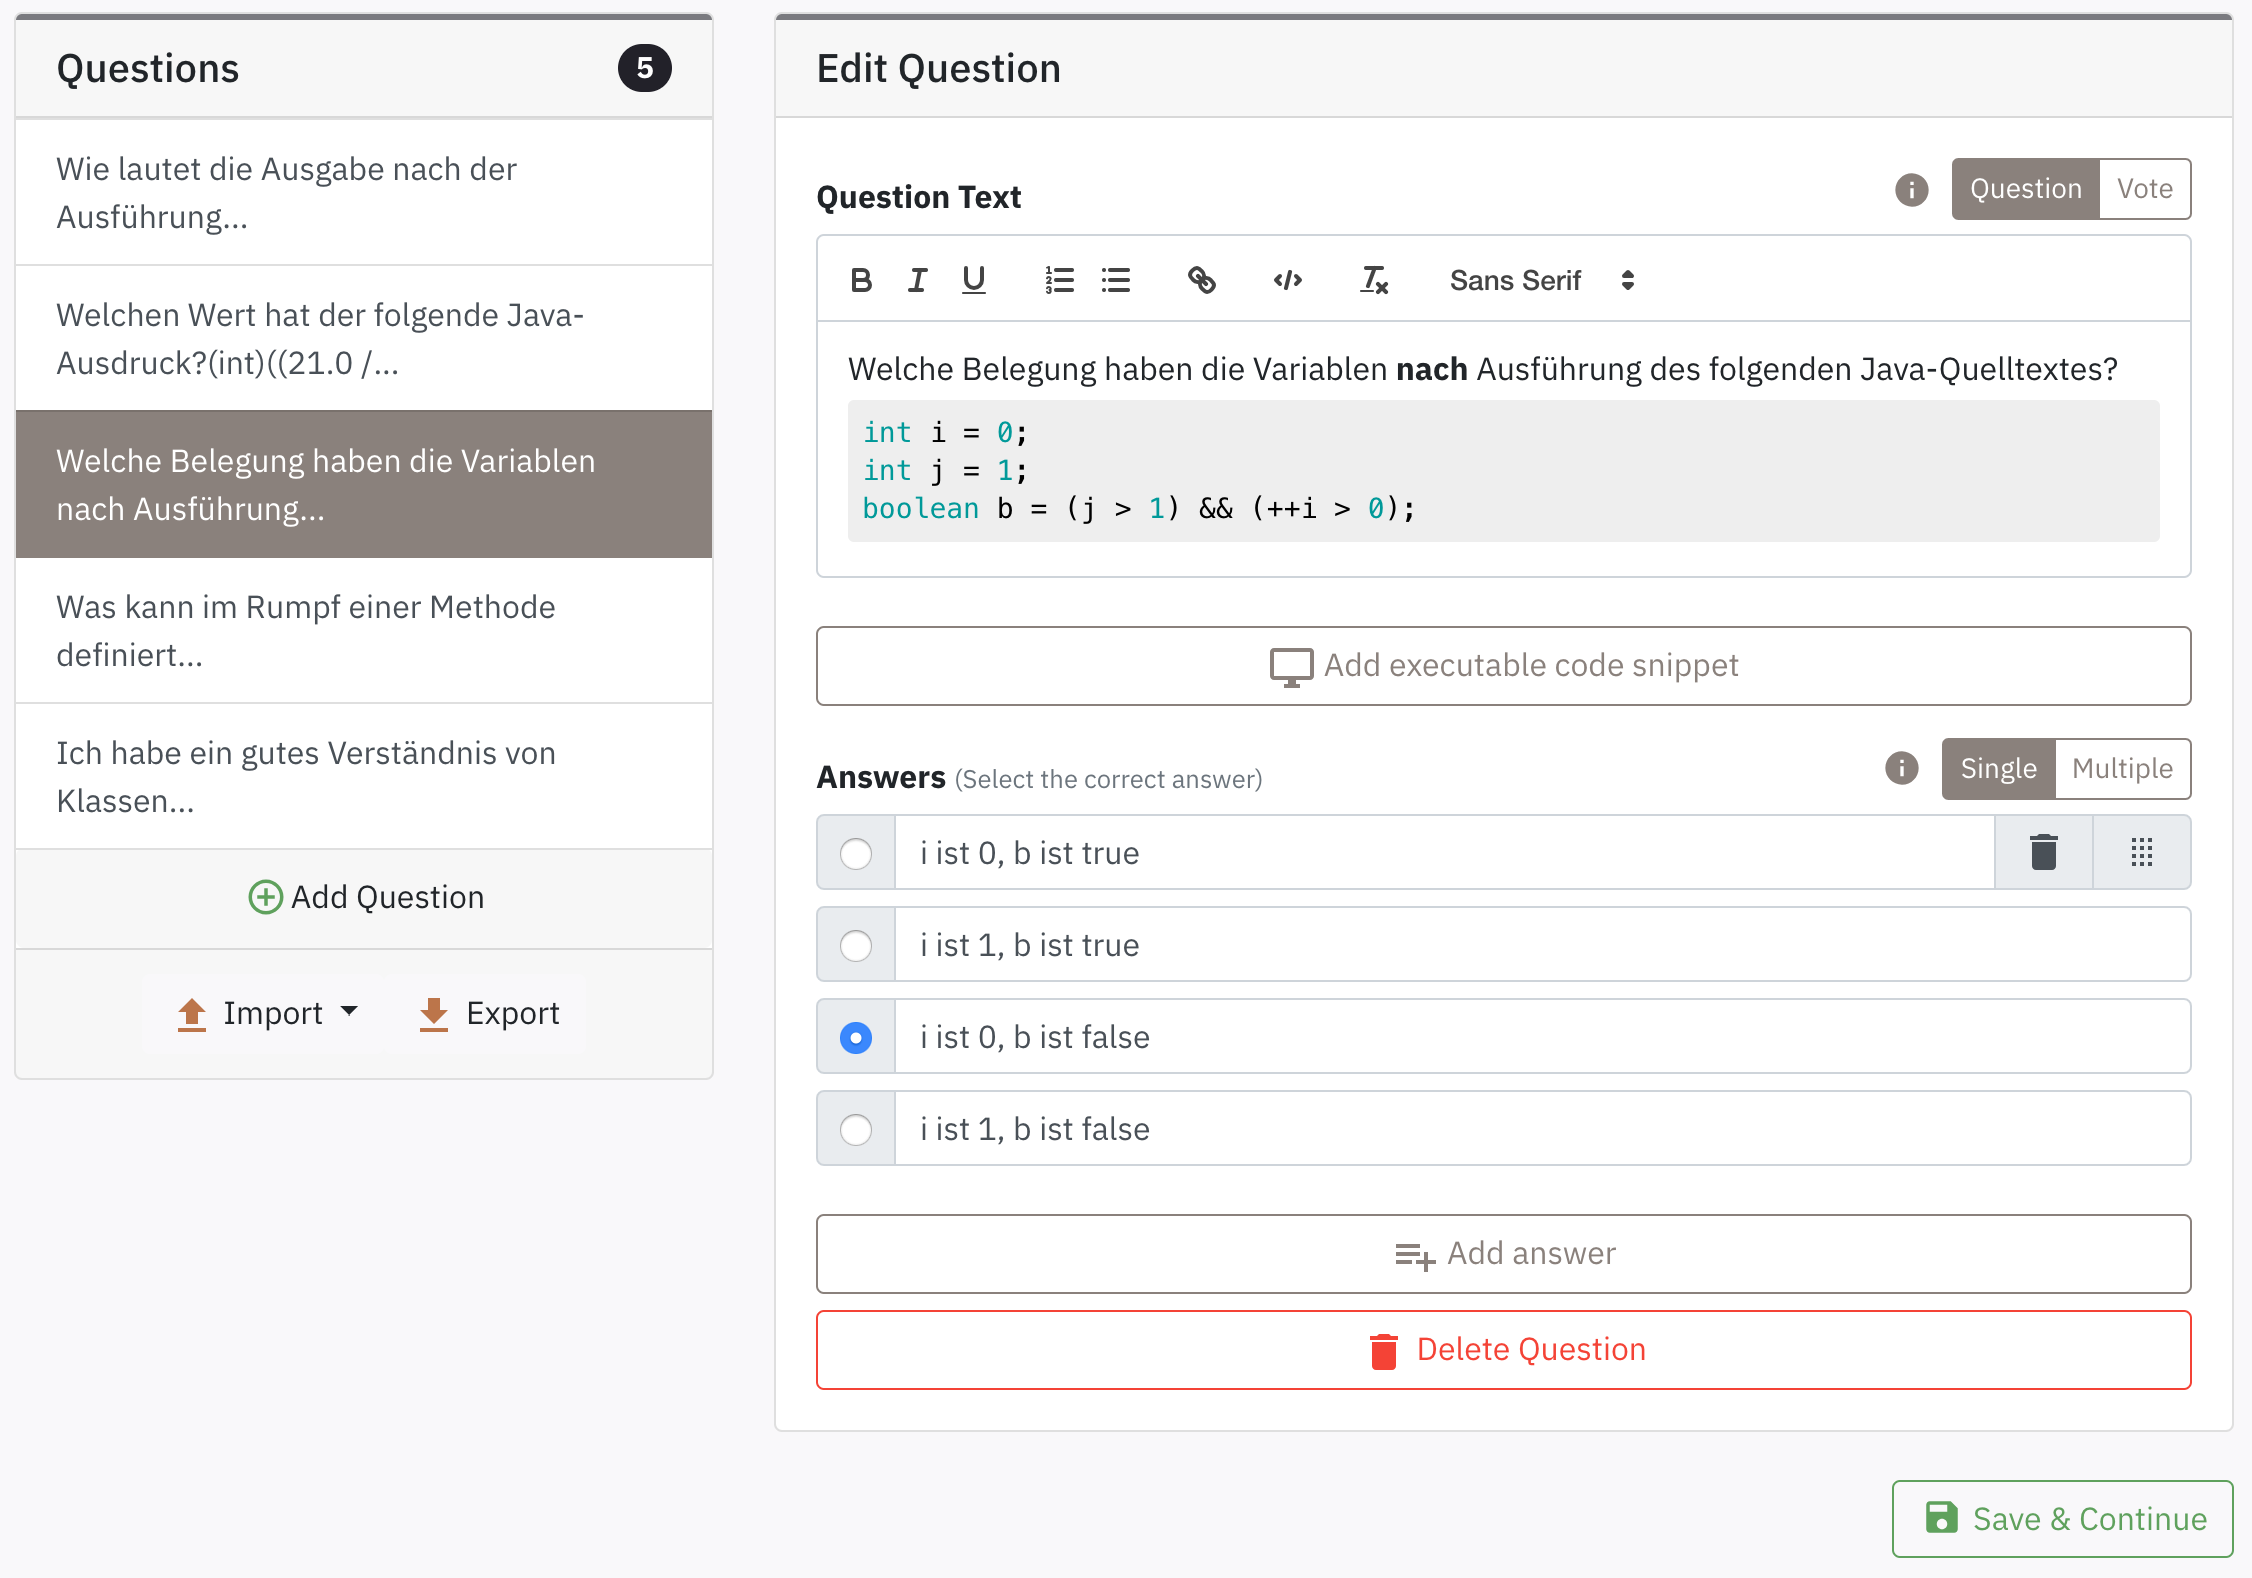
\includegraphics[width=\textwidth-1pt]{chapter/entwurf/bilder/weclare_editor.png}}
    \caption{Fertige Implementierung des Fragen-Editors im React-Framework.}
    \label{abb:weclare_editor}
\end{figure}

Alle Daten, mit denen der Fragen-Editor arbeitet, werden in einem einzigen Redux-Store gehalten. Alle möglichen Änderungen finden sich in einem zugehörigen Reducer wieder, der auszugsweise wie folgt aussieht:


\begin{minipage}{\linewidth}
\begin{lstlisting}[caption={Auszug aus dem Reducer für den Fragen-Editor (aus: src/server/reducers/questions.js)}]
export const questionEditor = (state = [], action) => {
  switch (action.type) {
    case ADD_QUESTION: {...}
    case EDIT_QUESTION_TEXT: {...}
    case EDIT_QUESTION_CODE: {...}
    case EDIT_QUESTION_MODE: {...}
    case EDIT_QUESTION_TYPE: {...}
    case DELETE_QUESTION: {...}
    case DELETE_ANSWER: {...}
    case ADD_ANSWER: {...}
    case EDIT_ANSWER_TEXT: {...}
    case SET_CORRECT_SINGLE_ANSWER: {...}
    case SET_CORRECT_MULTI_ANSWER: {...}
    case LOAD_QUESTIONS: {...}
    case SORT_QUESTION: {...}
    case SORT_ANSWER: {...}
    default: {
      return state;
    }
  }
};
\end{lstlisting}
\end{minipage}